\begin{figure}[t]
    \vspace*{-16px}
    \vspace*{-\figskipabove px}
    \centering
    {\scriptsize
    \begin{subfigure}[t]{0.235\textwidth}
        % 0
        \begin{subfigure}[t]{0.49\textwidth}
            \vspace{0px}\centering
            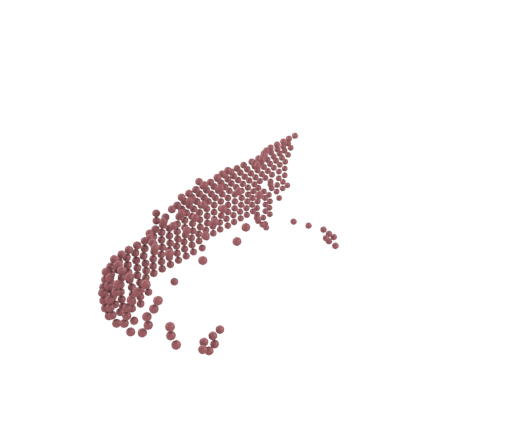
\includegraphics[width=2.25cm,trim={3cm 3cm 3cm 3cm},clip]{gfx_intro_shapenet_165_points}
        \end{subfigure}
        \begin{subfigure}[t]{0.49\textwidth}
            \vspace{0px}\centering
            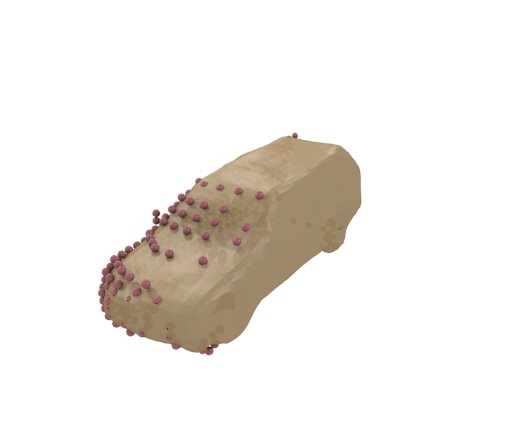
\includegraphics[width=2.25cm,trim={3cm 3cm 3cm 3cm},clip]{gfx_intro_shapenet_results_165}
        \end{subfigure}
        \vspace*{-2px}
        \subcaption{ShapeNet (Synthetic)}
    \end{subfigure}
    \begin{subfigure}[t]{0.235\textwidth}
        \begin{subfigure}[t]{0.49\textwidth}
            \vspace{0px}\centering
            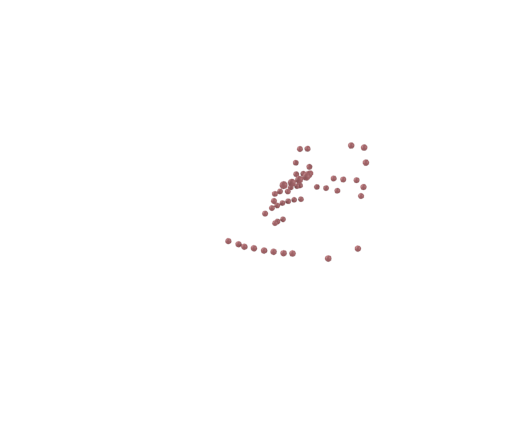
\includegraphics[width=2.25cm,trim={3cm 3cm 3cm 3cm},clip]{gfx_intro_kitti_1224_points}
        \end{subfigure}
        \begin{subfigure}[t]{0.49\textwidth}
            \vspace{0px}\centering
            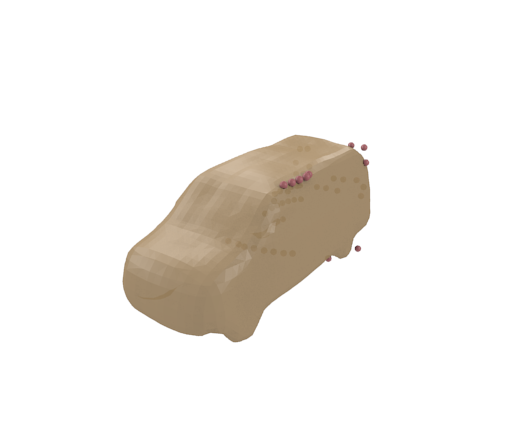
\includegraphics[width=2.25cm,trim={3cm 3cm 3cm 3cm},clip]{gfx_intro_kitti_results_1224}
        \end{subfigure}
        \subcaption{KITTI (Real)}
    \end{subfigure}
    \\[2px]
    % 2233
    \begin{subfigure}[t]{0.235\textwidth}
        % 264 1188 1452
        \begin{subfigure}[t]{0.49\textwidth}
            \vspace{0px}\centering
            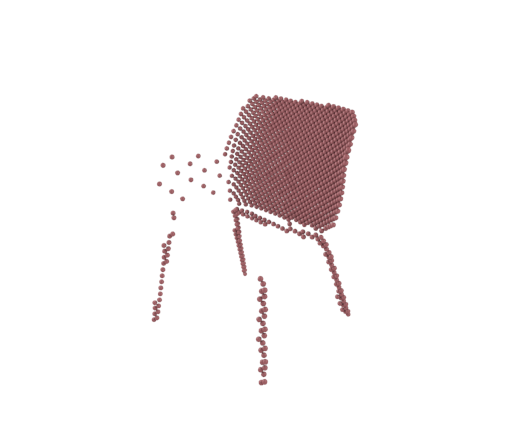
\includegraphics[width=2.25cm,trim={3cm 3cm 3cm 3cm},clip]{gfx_intro_modelnet_1452_points}
        \end{subfigure}
        \begin{subfigure}[t]{0.49\textwidth}
            \vspace{0px}\centering
            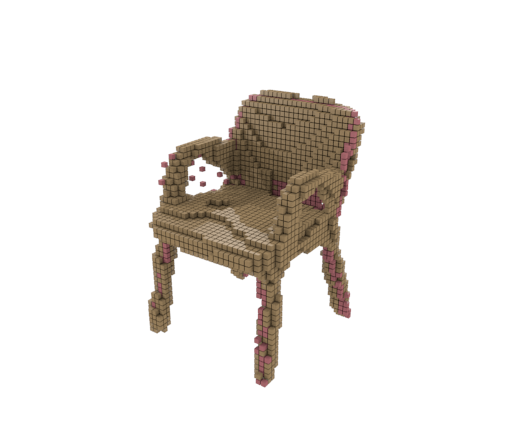
\includegraphics[width=2.25cm,trim={3cm 3cm 3cm 3cm},clip]{gfx_intro_modelnet_results_1452}
        \end{subfigure}
        \subcaption{ModelNet (Synthetic)}
    \end{subfigure}
    \begin{subfigure}[t]{0.235\textwidth}
        \begin{subfigure}[t]{0.49\textwidth}
            \vspace{0px}\centering
            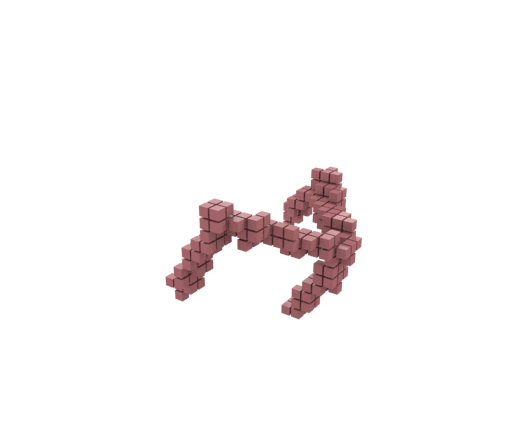
\includegraphics[width=2.25cm,trim={3cm 3cm 3cm 3cm},clip]{gfx_intro_yang_5_bin_points}
        \end{subfigure}
        \begin{subfigure}[t]{0.49\textwidth}
            \vspace{0px}\centering
            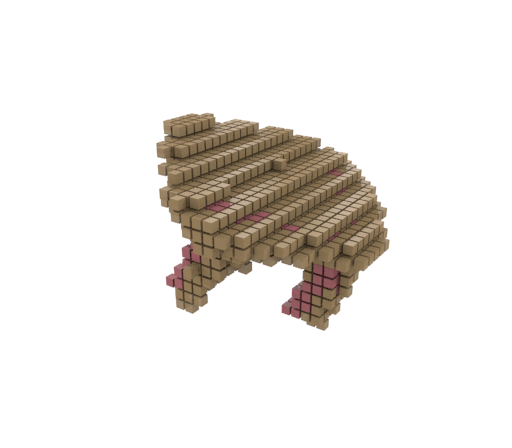
\includegraphics[width=2.25cm,trim={3cm 3cm 3cm 3cm},clip]{gfx_intro_yang_results_5}
        \end{subfigure}
        \subcaption{\Kinect (Real)}
    \end{subfigure}
    }
    \vspace*{-\figskipcaption px}
    \caption{{\bf 3D Shape Completion.} Results for cars on ShapeNet \citep{Chang2015ARXIV} and KITTI \citep{Geiger2012CVPR} and for chairs and tables on ModelNet \citep{Wu2015CVPR} and \Kinect \citep{Yang2018ARXIVb}. Learning shape completion on real-world data is challenging due to sparse and noisy observations and missing ground truth. Occupancy grids (bottom) or meshes from signed distance functions (SDFs, top) at various resolutions in {\color{rbeige}beige} and point cloud observations in {\color{rred}red}.}
    \label{fig:introduction}
    \vspace*{-\figskipbelow px}
\end{figure}